\chapter{Literature Review}
% Main Gist 
% - History of FHR reactor type and why there is a renewed interest in this
%   reactor type (start ups, labs etc.)
% - Past applications of AI to nuclear reactor design. 
% Structure 
% - Fluoride-Salt-Cooled High-Temperature Reactor (why salt cooled triso fuelled 
%   reactors are cool)
%   - FHR Modeling Challenges (why benchmark exists)
%   - Description of benchmark
% - Artificial Intelligence Applications to Nuclear Reactor Design Optimization
%   - Past work 
%   - Classical vs Evolutionary methods 

In this chapter, we provide a literature review of relevant past research 
efforts that give context to this proposed work. 
We begin with an overview of the \gls{FHR} concept, then go into detail about 
the specific \gls{AHTR} design, previous effort towards modeling the design and 
technical challenges faced, and a description of how these efforts led to the 
initiation of the \gls{OECD} \gls{NEA} \gls{AHTR} benchmark.  
Next, we outline the history of additive manufacturing and describe the current 
research towards application of additive manufacturing to fabrication of 
nuclear reactor core components. 
Next, we review previous efforts towards nuclear reactor design optimization 
and describe the impact of additive manufacturing advancements on reactor 
design optimization. 
Finally, we give a background of evolutionary algorithms and how they can be 
applied for optimizing reactor designs that are constructed with additive 
manufacturing technology.

\section{Fluoride-Salt-Cooled High-Temperature Reactor}
The \gls{FHR} is a reactor concept introduced in 2012 that uses high-temperature 
coated-particle fuel and a low pressure liquid fluoride-salt coolant 
\cite{forsberg_fluoride-salt-cooled_2012,facilitators_fluoride-salt-cooled_2013}.
\gls{FHR} technology combines the best aspects of \gls{MSR} and \gls{VHTR} 
(or \gls{HTGR}) technologies. 
Molten fluoride salts as working fluids for nuclear reactors have been explored 
since the 1960s and are desirable because of the salts' high-temperature 
performance and overall chemical stability \cite{scarlat_design_2014}.  
Using molten salts for reactor coolant introduces inherent safety compared 
to water due to the salts' high boiling temperature and high volumetric 
heat capacity, eliminating the risk of coolant boiling off, resulting in 
fuel elements overheating \cite{ho_molten_2013}. 
The leading candidate coolant salt is the fluoride salt Li$_2$BeF$_4$ (FLiBe), 
which remains liquid without pressurization up to 1400 $^{\circ}$C and a larger 
$\rho C_p$ than water \cite{ho_molten_2013,forsberg_fluoride-salt-cooled_2012}. 
\glspl{FHR} are favorable compared to a liquid fuel reactor, such as
\gls{MSR} systems, because the solid fuel cladding adds an extra barrier to fission 
product release 
\cite{ho_molten_2013}.

\gls{VHTR} technology has been studied since the 1970s because they delivers 
heat at substantially high temperatures than \glspl{LWR} resulting in 
the following advantages: increased power conversion efficiency, reduced 
waste heat generation, and co-generation and process heat capabilities 
\cite{scarlat_design_2014}. 
In \glspl{VHTR}, the helium coolant is held at a high pressure of approximately 
100 atm, whereas the \gls{FHR}'s FLiBe coolant is at room pressure, resulting in lower 
construction costs since a thick concrete reactor vessel is not required.
The molten salt coolant has superior cooling and moderating properties compared 
to helium coolant in \glspl{VHTR}, resulting in \glspl{FHR} operating at 
power densities two to six times higher than  \glspl{VHTR} 
\cite{scarlat_design_2014,forsberg_fluoride-salt-cooled_2012}.
Therefore, by combining the FLiBE coolant from \gls{MSR} technology and 
\gls{TRISO} particles from \gls{VHTR} technology, the \gls{FHR} benefits from 
the low operating pressure and large thermal margin provided by using a molten 
salt coolant and the accident-tolerant qualities of \gls{TRISO} particle fuel. 

There are several types of \gls{FHR} conceptual designs that exist
worldwide: \gls{PBFHR} at UCB with circulating pebble-fuel 
\cite{scarlat_current_2014,krumwiede_three-dimensional_2013}, the \gls{SF-TMSR} 
at the \gls{SINAP} in China with static pebble-fuel \cite{liu_preliminary_2016}, 
the large central-station \gls{AHTR} at \gls{ORNL} \cite{holcomb_core_2011, varma_ahtr_2012} and 
the \gls{SmAHTR} at ORNL \cite{greene_pre-conceptual_2010} with static plate-fuel. 

\subsection{AHTR design}
This proposed work is focused on the FHR design with hexagonal fuel elements 
consisting of \gls{TRISO} fuel particles embedded in plates ("planks"), i.e., the 
\gls{AHTR} design developed by ORNL. 
The \gls{AHTR} has 3400 MWt thermal power and 1400 MW electric power with
inlet/outlet temperatures of 650/700$^{\circ}C$ \cite{varma_ahtr_2012}. 
The prismatic \gls{AHTR}'s fuel element and core configuration are shown in 
Figure \ref{fig:ahtr}.  
Each hexagonal fuel element features plate-type fuel consisting of eighteen plates 
arranged in three diamond-shaped sectors, with a central Y-shaped structure 
and external channel (wrapper).
Each fuel plank is made of an isostatically pressed carbon with fuel stripes 
on each outer side of the plank. 
The fuel stripes are prismatic regions composed of a graphite matrix filled with 
a cubic lattice of \gls{TRISO} particles. 
The core consists of 252 assemblies radially surrounded by reflectors
\cite{ramey_monte_2018}. 
Chapter \ref{chap:fhr-benchmark} details the specifications of the AHTR geometry
modeled in this proposed work.

\begin{figure}[H]
    \centering
    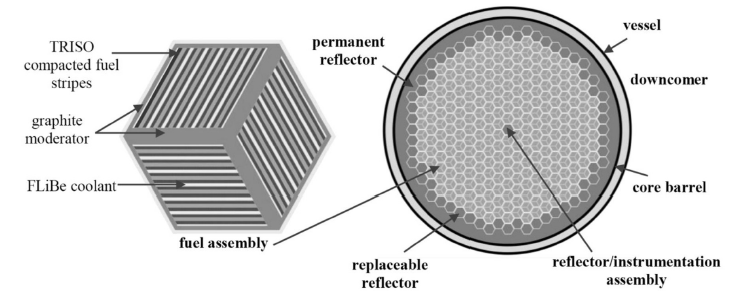
\includegraphics[width=0.9\linewidth]{ahtr.png} 
    \caption{FHR core configuration and fuel element \cite{ramey_monte_2018}.}
    \label{fig:ahtr}
\end{figure}

\subsection{Previous AHTR modeling efforts and challenges}
Modeling and simulation of the \gls{AHTR} design has been an ongoing effort 
since its conception in 2003 \cite{forsberg_molten-salt-cooled_2003}. 
The \gls{AHTR} core design differs significantly from the present \gls{LWR}-based 
nuclear power plants. 
These differences lead to modeling challenges and the need for verification and 
validation of modeling and simulation methods \cite{ramey_monte_2018}. 
Verification and validation of neutronics and thermal hydraulics tools' 
capability to successfully model the \gls{AHTR} design is a crucial step 
in support of licensure of the \gls{AHTR} design towards the eventual goal 
of deployment \cite{rahnema_phenomena_2019,rahnema_current_2015}. 
Several neutronic studies have been completed along the way to the current 
\gls{AHTR} design \cite{ramey_monte_2018,holcomb_fluoride_2013,greene_pre-conceptual_2010}. 
These efforts have shed light on the technical challenges facing the \gls{AHTR} design. 

In an effort to understand the challenges of \gls{FHR} materials, 
modeling the neutronics and thermal hydraulics in 
both plate and pebble fuelled \glspl{FHR}, a university-led Integrated 
Research Project \cite{zhang_integrated_2019} was conducted. 
During the research project, a panel of subject matter experts came together to 
generate a \gls{PIRT} by identifying phenomena and ranking their importance.
The \gls{PIRT} identifies areas in which additional research is needed to better 
understand important phenomena for adequate future modelling 
\cite{rahnema_phenomena_2019}. 
The phenomena identified as requiring further research are included in 
Table \ref{tab:phenomena}. 

\begin{table}[]
    \centering
    \onehalfspacing
    \caption{\gls{PIRT} identified \gls{FHR} physical phenomena requiring further research 
    \cite{rahnema_phenomena_2019}.}
	\label{tab:phenomena}
    \small
    \begin{tabular}{l|l}
    \hline
    \textbf{Category} & \textbf{Phenomena} \\ \hline
    Fundamental cross section data & - Moderation in FliBe \\
    & - Thermalization in FliBe \\
    & - Absorption in FliBe \\
    & - Thermalization in carbon \\
    & - Absorption in carbon \\ \hline
    Material Composition & - Fuel particle distribution \\ \hline
    Computational Methodology & - Solution Convergence \\ 
    & - Granularity of depletion regions \\
    & - Multiple heterogeneity treatment for generating multi-group \\ 
    & cross sections \\
    & - Selection of multi-group structure \\
    & - Boundary conditions for multi-group cross section generation \\ \hline 
    General Depletion & Spectral history \\ \hline 
    \end{tabular}
    \end{table}

The \gls{AHTR} has a complex core design due to the multiple heterogeneity present 
in the fuel introduced by presence of \gls{TRISO} particles embedded in plates 
\cite{ramey_monte_2018,rahnema_phenomena_2019}.
Accurately modeling the \gls{FHR}'s complex geometry with individual \gls{TRISO}
particle fidelity is necessary to obtain detailed reference power distributions 
to assess the accuracy of lower-fidelity models.
However, it is challenging, particularly for deterministic codes which 
use multigroup cross sections and traditional homogenization methods
\cite{ramey_monte_2018}. 
These traditional homogenization methods are insufficient to capture the correct physics 
in \glspl{FHR}, due to the multiple heterogeneity \cite{ramey_monte_2018}. 
In the \gls{AHTR}, single and multiple slab homogenization decreased computation time 
by 10, however they introduce a nontrivial error of $\sim$3\%
\cite{ramey_monte_2018,cisneros_neutronics_2012}.
Core physics parameters with acceptable uncertainty must be calculated to determine 
the feasibility and safety of the \gls{AHTR} design.
For Monte Carlo codes, statistical uncertainties must be reduced by increasing 
the number of neutron histories, however this comes at an increased 
computational cost.

Another technical challenge faced by the \gls{AHTR} design is the uncertainty of 
the graphite and carbonaceous moderator material properties: densities, temperatures
and thermal scattering data.
Also, the thermal scattering data ($S(\alpha,\beta)$ matrices) for the bound 
nuclei in the \gls{FLiBe} salt are lacking \cite{ramey_monte_2018}. 
Upon examination of the thermal scattering behavior of solid \gls{FLiBe}
\cite{mei_investigation_2013} and liquid \gls{FLiBe} \cite{zhu_thermal_2017}, 
it was observed that the bound and free atom cross section of \gls{FLiBe} are 
identical above 0.1eV and diverges below 0.01eV. 
This means that the use or absence of thermal scattering data will impact the 
accuracy of the results \cite{ramey_monte_2018}. 

\subsection{AHTR Benchmark}
In an effort to address and further understand the technical challenges described 
in the previous section, in 2019 the OECD-NEA initiated a benchmark to assess the 
state of the art modelling and simulation capabilities for \glspl{FHR} with 
\gls{TRISO} fuel embedded in fuel plates ("planks") of hexagonal fuel elements
\cite{noauthor_fluoride_nodate}. 
The benchmark plans to have three phases, starting from a single fuel element 
simulation without burnup, gradually extending to full core depletion and feedback. 
The overarching objective of the benchmark is to identify applicability, accuracy, 
and practicality of the current methods and codes to assess the current state 
of the art of \gls{FHR} simulation and modeling \cite{petrovic_preliminary_2021}. 
The benchmark also enables the cross-verification of codes and methodologies for the 
challenging \gls{AHTR} geometry, which is especially useful since applicable reactor 
physics experiments that may be used for validation of codes are scarce  
 \cite{petrovic_fhrahtr_2019,petrovic_preliminary_2021}. 
A detailed description of the phases of the benchmark and the results to date 
are described in Chapter \ref{chap:fhr-benchmark}. 

\section{Additive Manufacturing}
\gls{AM} is the formalized termed for what used to be called rapid prototyping 
and what is popularly called 3D printing \cite{gibson_additive_2014}. 
The basic principle of \gls{AM} is that a model is initially generated using a
\gls{3D CAD} system and is fabricated directly without the need for process 
planning. 
In \gls{AM}, the parts are made by adding materials in layers, each layer is a 
thin cross-section of the \gls{3D CAD} designed part, as opposed 
to subtractive manufacturing methods such as traditional machining
\cite{standard_standard_2012}. 
All commercialized \gls{AM} machines to date use a layer-based approach, and 
the major ways that they differ are in the materials that can be used, 
how the layers are created, and how the layers are bonded to each other
\cite{gibson_additive_2014}.
These major differences will determine the following factors: accuracy of the 
final part, its material and mechanical properties, time required to manufacture 
the part, the need for post-processing, size of \gls{AM} machine, and overall 
cost of the machine and the process \cite{gibson_additive_2014}. 
Initially, \gls{AM} was used to manufacture prototypes. 
However, with improvements in material properties, accuracy and overall quality 
of \gls{AM} output, the applications for \gls{AM} expanded, to the 
current point in which some industries build parts for direct assembly purposes
\cite{uriondo_present_2015}.  
Furthermore, using \gls{AM} in conjunction with other technologies, such as 
high-power laser technology, has enabled the use of \gls{AM} technology 
to manufacture parts made from a variety of metals \cite{gibson_additive_2014}. 

\subsection{Application of Additive Manufacturing to Nuclear Reactor Core Components}
\label{sec:am}
\gls{AM} has progressed rapidly in the last 30 years from rapid design protoyping 
with polymers in the automotive industry to scale production of metal components.  
Examples include Boeing using \gls{AM} to reduce the 979 Dreamliner's weight 
\cite{noauthor_printed_2017} and General Electric using \gls{AM} to produce fuel 
injection nozzles \cite{noauthor_transformation_2018}. 
The most common metal \gls{AM} technologies, \gls{SLM}, \gls{EBM}, \gls{L-DED}, 
and binder jetting, are not currently used to manufacture nuclear power plant parts. 
Wide-spread adoption of these methods in the nuclear industry could drastically 
reduce fabrication costs and timelines, combine multiple systems and assembled 
components into single parts, increase safety and performance by tailoring 
local material properties, and allow for redesigning of geometries for optimal 
load paths \cite{simpson_considerations_2019}. 
Many generation IV advanced reactor concepts have complex geometries, 
such as hex-ducts for sodium-cooled fast reactors, which are costly and difficult 
to fabricate using common processing techniques. 
Traditional manufacturing routes also restrict the viable geometries for 
reactor designers \cite{sridharan_performance_2019}. 
In summary, the main benefits of using \gls{AM} for reactor core components is that 
we are no longer geometrically constrained by conventional fuel manufacturing, 
and can further optimize and improve fuel geometries to enhance fuel performance and 
safety with the added benefit of lower cost \cite{bergeron_early_2018}. 

There has been experimental work done in the nuclear materials field towards 
demonstration of \gls{AM} of nuclear fuel and structural core materials. 
Bergeron et al \cite{bergeron_early_2018} successfully demonstrated additively 
manufacturing thorium dioxide using a stereolithography-based 3D printer 
and photopolymer resin. 
The high-density thorium dioxide objects were printed and sintered to densities 
of $\sim90\%$ \cite{bergeron_early_2018}. 
Rosales et al \cite{rosales_characterizing_2019} conducted a feasibility study 
of direct routes to fabricate dense uranium silicide ($U_3Si_2$) fuel pellets 
using the \gls{INL} invented \gls{AMAFT}. 
$U_3Si_2$ is an accident-tolerant nuclear fuel candidate due to its promising 
high uranium density and improved thermal properties. 
Its current metallurgical fabrication process is expensive and long, the goal of
\gls{AMAFT} is to fabricate $U_3Si_2$ at a lower cost, in a timely and
commercially-reliable manner \cite{rosales_characterizing_2019}.  
Sridharan et al \cite{sridharan_performance_2019} demonstrated the application of
the laser-blown-powder \gls{AM} process to fabricate \gls{FM} steel, a type of 
steel commonly used for cladding and structural components in nuclear reactors. 
Koyanagi et al \cite{koyanagi_additive_2020} presented the current status of 
\gls{AM} technology for manufacturing nuclear-grade \gls{SiC} materials, they 
demonstrated that combinations of \gls{AM} techniques and traditional \gls{SiC} 
densification methods enabled new designs of \gls{SiC} components with complex shapes. 
\gls{SiC} has excellent strength at elevated temperatures, chemical inertness, 
relatively low neutron absorption, and stability under neutron irradiation up 
to high doses \cite{sauder_ceramic_2014, snead_handbook_2007,koyanagi_additive_2020} 
which make it suitable for many applications in nuclear systems such as fuel cladding, 
constituents of fuel particles \cite{snead_handbook_2007} and pellets
\cite{terrani_progress_2015}, core structural components in fission reactors 
\cite{sauder_ceramic_2014}. 

\section{Nuclear Reactor Design Optimization}
\label{sec:opt}
The practice of nuclear reactor optimization has been around since the conception of 
nuclear reactors. 
Optimization has been applied to nuclear reactor design, reactor reloading 
patterns, and the nuclear fuel cycle.  
In the proposed work, we will focus on the optimization of nuclear reactor 
core design. 
Previous efforts towards nuclear reactor core design optimization include the use 
of deterministic and stochastic optimization techniques, and these optimization 
methods coupled with surrogate models. 

Deterministic optimization methods usually start from a guess solution, 
thereafter the algorithm suggests a search direction based on applying local 
information to a pre-specified transition rule. 
The best solution becomes the new solution and the above procedure is continued 
for a number of times \cite{deb_multi-objective_2001}. 
Drawbacks of deterministic methods include: algorithms tend to get stuck to a 
suboptimal solution and an algorithm efficient in solving one type of problem, 
may not be efficient in solving a different problem \cite{deb_multi-objective_2001}. 
Stochastic optimization methods minimize or maximize an objective function 
when randomness is present, they tend to find globally optimal solutions 
more reliably than deterministic methods. 
Evolutionary algorithms and simulated annealing are examples of stochastic 
optimization algorithms. 

The complexity of a nuclear reactor results in reactor design optimization 
being a multi-objective design problem requiring a tradeoff between desirable 
attributes \cite{byrne_evolving_2014,simon_sciences_2019}. 
When multiple conflicting objectives are important, there is no single optimum 
solution which simultaneously optimizes all objectives. 
Instead, the multi-objective optimization problem's outcome is a set of optimal 
solutions with a varying degree objective values \cite{deb_multi-objective_2001}. 
For a multi-objective problem like reactor design optimization, 
an ideal multi-objective optimization method should find widely spread solutions 
in the obtained non-dominated front \cite{deb_multi-objective_2001}. 

Recent efforts towards nuclear reactor optimization have relied heavily on 
stochastic methods such as simulated annealing and evolutionary algorithms, 
with occasional addition of stochastic-deterministic hybrid methods. 
Sacco et al \cite{sacco_two_2006,sacco_metropolis_2008} used stochastic 
optimization techniques similar to simulated annealing, and a 
deterministic-stochastic hybrid optimization technique
that combined one of the stochastic simulated annealing methods with the 
deterministic Nelder–Mead Simplex algorithm to optimize reactor dimensions, 
enrichment, materials etc., in order to minimize the average peak factor in a 
three-enrichment-zone reactor. 
Odeh et al \cite{odeh_core_2016} used the simulated annealing stochastic algorithm 
coupled with neutronics and thermal hyraulics codes, \gls{PARCS} and RELAP5, 
to develop an optimum core design for the \gls{NMR-50} to achieve a 10-year cycle length 
with minimal fissile loading. 
Kropaczek et al \cite{kropaczek_large-scale_2019} demonstrated the constraint 
annealing method, a highly scalable method based on the method of parallel 
simulated annealing with mixing of states \cite{kropaczek_constraint_2019}, for 
the solution of large-scale, multiconstrained problems in \gls{LWR} fuel cycle 
optimization. 
Peireira et al \cite{pereira_coarse-grained_2003,pereira_parallel_2008} 
used a coarse-grained parallel \gls{GA} and a niching \gls{GA}
to optimize the same problem as \cite{sacco_two_2006}. 
Kamalpour et al \cite{kamalpour_smart_2020} utilized the imperialist competitive 
algorithm, a type of evolutionary algorithm, to optimize a \gls{FCM} fuelled 
\gls{PWR} to extend the reactor core cycle length. 

Nuclear reactor optimization problems require the use of computationally 
extensive neutronics and thermal-hydraulics software to compute the objective 
function and constraints. 
In an effort to reduce computational cost of utilizing stochastic methods, 
multiple papers utilized optimization methods with surrogate models to replace 
high fidelity neutronics or thermal hydraulics simulations that typically 
require a high computational cost. 
Kumar et al \cite{kumar_new_2015} combined genetic algorithm optimization 
with regression splines surrogate model to optimize a reactor model for 
high breeding of U-233 and Pu-239 in desired power peaking limits, desired 
keff using the following parameters: radius of a fuel pin cell, isotopic enrichment 
of the fissile material in the fuel, mass flow rate of the coolant, and temperature 
of the coolant at the core inlet.
Betzler et al \cite{betzler_design_2019} developed a systematic approach to 
build a surrogate model to serve in place of high-fidelity computational 
analyses, they then leveraged the surrogate model with a simulated annealing 
optimization algorithm to generate optimized designs at a lower computational 
cost to understand the impact of design decisions on desired metrics for 
\gls{HFIR} \gls{LEU} core designs. 

The simulation annealing method uses a point-by-point approach, in which one
solution gets updated to a new solution in one iteration, which does not 
allow for advantages of parallel systems to be fully exploited. 
Finding an optimal solution with simulation annealing methods will take very 
long if high-fidelity computationally expensive codes are used to compute 
the objective function and constraints.
Therefore, using the simulation annealing method is only practical if a 
surrogate evaluation model is used as described in \cite{betzler_design_2019}
and \cite{kumar_new_2015}.
Evolutionary algorithm method mimics nature's evolutionary principles to drive 
its search towards an optimal solution. 
Contrary to a single solution per iteration in deterministic and the stochastic 
simulation annealing methods, \glspl{EA} use a population of solutions in each 
iteration \cite{deb_multi-objective_2001}. 
With the affordability and availability of parallel computing systems, the 
evolutionary algorithm optimization method stands out as a method 
that easily and conveniently exploits parallel systems. 
Further, \glspl{EA} have proved amenable to \gls{HPC} solution and 
scalable to tens of thousands of processors \cite{kropaczek_constraint_2019}. 
Therefore, in this proposed work, we will utilize the evolutionary algorithm 
optimization method. 

\subsection{Impact of additive manufacturing on nuclear reactor design 
optimization}
In section \ref{sec:am}, we discussed how with the advancements of \gls{AM} 
for reactor core components, reactor designers are no longer geometrically 
constrained by conventional fuel manufacturing, and can further optimize and 
improve fuel geometries to enhance fuel performance and safety. 
Reactor design objectives remain consistent with past objectives, such as minimizing 
fuel amount, minimizing maximum fuel temperature for a given power level. 
However, we can now approach the nuclear design problems with truly arbitrary 
geometries, no longer limited by traditional geometric shapes that are 
easy to manufacture with traditional processes: slabs as fuel plates, cylinders 
as fuel rods, spheres as fuel pebbles, axis-aligned coolant channels, etc  
\cite{sobes_artificial_2020}.
Therefore, this has opened the door for re-examination of optimization in 
completely new way, determining the optimal arbitrary geometry for a given objective 
function \cite{sobes_artificial_2020} with a much smaller set of constraints. 

With a substantial increase and change in the design space of an arbitrary 
geometry, it becomes time consuming for a human reactor designer to completely 
explore the design space to find optimal geometries. 
Instead, we can leverage \gls{AI} optimization methods such as \gls{EA} to 
effectively explore the large design space in a timely manner to find global 
optimal designs. 
\gls{AI} would not replace the human reactor designer, but will shift the 
human designer's focus away from conjecturing good geometries to defining 
design criteria to find optimal designs \cite{sobes_artificial_2020}. 
Therefore, when the human designer changes the reactor criteria, the \gls{AI} 
model will easily adapt and produce new global optimal designs to fit the new 
criteria.  

\section{Evolutionary Algorithms} 
\glspl{EA} mimic natural evolutionary principles to constitute search and 
optimization procedures \cite{deb_multi-objective_2001}.  
The most popular \glspl{EA} used to solve multi-objective 
problems are genetic algorithms (GA) 
\cite{byrne_evolving_2014, krish_practical_2011}. 

\subsection{Genetic Algorithms}
\glspl{GA} imitate natural genetics and selection to evolve solutions 
by (1) maintaining a population of solutions, (2) allowing 
fitter solutions reproduce, and (3) letting lesser fit solutions die off, 
resulting in final solutions that are better than the previous generations 
\cite{renner_genetic_2003}. 
From here, we will refer to a solution as an individual within the population. 
They efficiently exploit historical information to speculate new search 
points with expected improved performance \cite{goldberg_genetic_1989}. 
\glspl{GA} are theoretically and empirically proven to provide robust 
search in complex spaces and are computationally simple yet powerful 
in their search for improvement \cite{goldberg_genetic_1989}. 
As discussed in section \ref{sec:opt}, \glspl{GA} are advantageous compared to 
deterministic and other stochastic optimization methods, such as simulated 
annealing because it searches from a population of points, uses objective 
function information, not derivatives or other auxillary knowledge of the 
problem, and uses probabilistic transition rules, not deterministic rules. 
Figure \ref{fig:genetic_alg} depicts the iterative process of using a \gls{GA}
to solve a problem. 
When a population does not meet termination criteria, a new generation is 
created. 
This occurs iteratively till the termination criteria is met.

\begin{figure}[!htbp]
        \centering
        \begin{tikzpicture}[node distance=1.7cm]
                \tikzstyle{every node}=[font=\small]
                \node (1) [lbblock] {\textbf{Create initial population}};
                \node (2) [lbblock, below of=1] {\textbf{Evaluate initial population}};
                \node (3) [loblock, below of=2, yshift = -1.3cm] {\textbf{Create new population:} \\ 
                \begin{enumerate} \item \textbf{select} individuals for mating 
                                  \item create offspring by \textbf{crossover} 
                                  \item \textbf{mutate} selected individuals 
                                  \item keep selected individuals from previous generation
                                 \end{enumerate}};
                \node (4) [loblock, below of=3, yshift=-1.3cm] {\textbf{Evaluate new population}};
                \node (5) [loblock, below of=4] {\textbf{Is termination criteria satisfied?}};
                \node (6) [lbblock, below of=5] {\textbf{Best solution is returned!}};
                \draw [arrow] (1) -- (2);
                \draw [arrow] (2) -- (3);
                \draw [arrow] (3) -- (4);
                \draw [arrow] (4) -- (5);
                \draw [arrow] (5) -- node[anchor=east] {Yes} (6);
                \draw [arrow] (5) -- ([shift={(0.5cm,0cm)}]5.east)-- node[anchor=west] {no} ([shift={(0.5cm,0cm)}]3.east)--(3);
        \end{tikzpicture}
        \caption{Process of solving a problem with genetic algorithm 
        \cite{renner_genetic_2003}. }
        \label{fig:genetic_alg}
\end{figure}

% explain how individuals look like 

\glspl{GA} are usually composed of three operators: selection, crossover, 
and mutation. 

\subsubsection{Selection Operator}
The selection operator's primary objective is to make duplicates of good 
individuals and eliminate bad individuals in a population, while keeping the 
population constant \cite{deb_multi-objective_2001}. 
It achieves this by identifying above-average individuals in a population and 
eliminating bad individuals from the population and replace them with copies 
of good individuals. 
Selection operator methods utilized in the proposed work include: tournament 
selection, best selection, and NSGA-II selection. 
In tournament selection, tournaments are played between a user-defined number 
of individuals and the best individual is kept in the population. 
This occurs repeatedly until all the population's spots are filled. 
In best selection, a user-defined number of best individuals are selected 
and copies of them are made to keep population size constant. 
In NSGA-II selection, parent and offspring populations are combined and the
best individuals (with respect to fitness and spread) are selected
\cite{deb_fast_2002}, and copies of the best individuals are made to keep 
population size constant. 

The selection operator cannot create any new individuals in the population, 
and only makes more copies of good individuals at the expense of not-so-good
individuals. 
The creation of new solutions is performed by the crossover and mutation 
operators. 

\subsubsection{Crossover Operator}
The crossover operator is also known as the mating operator. 
In most crossover operators, two individuals are picked from the population at 
random and some portion of the individuals' attributes are exchanged with one 
another to create two new individuals \cite{deb_multi-objective_2001}. 
Crossover operator methods utilized in the proposed work include: single-point
crossover, uniform crossover, and blend crossover. 
In single-point crossover, two individuals are selected from the population and 
a site along the individual's definition is randomly chosen. 
Attributes on the right side of this cross site are exchanged between the two 
individuals, creating two new offspring individuals.  
In uniform crossover, the user defines an independent probability for each 
individual attribute to be exchanged, usually $p=0.5$ is used. 
In blend crossover, two offspring (O) individuals are created based on a linear 
combination of two parent (P) individuals using the following equations: 

\begin{align}
    O_1 &= P_1 - \alpha(P_1-P_2) \\
    O_2 &= P_2 + \alpha(P_1-P_2)
\intertext{where}
\alpha &= \mbox{Extent of the interval in which the new values can be drawn} \nonumber \\
 & \mbox{for each attribute on both side of the parents’ attributes (user-defined)} \nonumber 
\end{align}

In order to preserve some good individuals selected during the selection 
operator stage, not all individuals are used in a crossover, this is implemented 
by having the user define a crossover probability ($p_c$).  
Therefore, the crossover operator is only applied to $100p_c\%$ of the 
population, the rest are simply copied to the new population
\cite{deb_multi-objective_2001}. 

\subsubsection{Mutation Operator}
